\documentclass[12pt,letterpaper]{article}

% ==============================================================================
% INF8770 - Technologies Multimédias - Polytechnique Montréal
% Gabarit officiel réutilisable pour les Travaux Pratiques (TP1, TP2, TP3, TP4)
% ==============================================================================

% ------------------------------------------------------------------------------
% Paquets requis
% ------------------------------------------------------------------------------
\usepackage[utf8]{inputenc}
\usepackage[T1]{fontenc}
\usepackage[french]{babel}
\usepackage{newtxtext,newtxmath}
\usepackage[margin=2cm]{geometry}
\usepackage{graphicx}
\usepackage{booktabs}
\usepackage{amsmath}
\usepackage{listings}
\usepackage{xcolor}
\usepackage{hyperref}
\usepackage{caption}
\usepackage{microtype}
\usepackage{float}
\usepackage{csvsimple}

% ------------------------------------------------------------------------------
% Configuration des liens hypertexte
% ------------------------------------------------------------------------------
\hypersetup{
    colorlinks=true,
    linkcolor=black,
    citecolor=blue!70!black,
    urlcolor=blue!80!black
}

% ------------------------------------------------------------------------------
% Configuration de listings pour le code source (Annexe)
% ------------------------------------------------------------------------------
\definecolor{codegreen}{rgb}{0,0.6,0}
\definecolor{codegray}{rgb}{0.5,0.5,0.5}
\definecolor{codepurple}{rgb}{0.58,0,0.82}
\definecolor{backcolour}{rgb}{0.97,0.97,0.97}

\lstdefinestyle{mystyle}{
    backgroundcolor=\color{backcolour},   
    commentstyle=\color{codegreen},
    keywordstyle=\color{blue}\bfseries,
    numberstyle=\tiny\color{codegray},
    stringstyle=\color{codepurple},
    basicstyle=\ttfamily\footnotesize,
    breakatwhitespace=false,         
    breaklines=true,                 
    captionpos=b,                    
    keepspaces=true,                 
    numbers=left,                    
    numbersep=7pt,                  
    showspaces=false,                
    showstringspaces=false,
    showtabs=false,                  
    tabsize=4,
    frame=single,
    rulecolor=\color{black!20}
}
\lstset{style=mystyle}

\begin{document}

% ==============================================================================
% PAGE DE TITRE (Gabarit officiel)
% ==============================================================================
\pagenumbering{roman}
\begin{titlepage}
    \centering
    \vspace*{0.5cm}
    
    % Logo officiel de Polytechnique Montréal
    
\includegraphics[width=0.45\textwidth]{logo_polytechnique.png}\\[1.5cm]
    
    {\Huge \textbf{INF8770 : Technologies Multimédias}}\\[0.5cm]
    {\LARGE \textbf{TP1 : Compression sans perte: texte}}\\[0.3cm]
    {\Large Automne 2026}\\[2cm]
    
    {\large \textbf{Étudiants :}}\\[0.3cm]
    {\normalsize Capistran-Champoux, Charlotte \quad (Matricule : 2353263)}\\[0.15cm]
    {\normalsize Nom Prénom Étudiant 2 \quad (Matricule : XXXXXXX)}\\[1.5cm]
    
    {\large \textbf{Chargé de laboratoire :}}\\[0.3cm]
    {\normalsize Nom du Chargé de Laboratoire}\\[2cm]
    
    \vfill
    
    {\normalsize Département de génie informatique et génie logiciel}\\
    {\normalsize Polytechnique Montréal}\\[0.5cm]
    {\small Date de remise : 28 septembre 2026 à 17h00 sur Moodle}
    
    \thispagestyle{empty}
\end{titlepage}

% ==============================================================================
% TABLE DES MATIÈRES
% ==============================================================================
\newpage
\pagenumbering{arabic}
\setcounter{page}{1}
\tableofcontents
\newpage

% ==============================================================================
% 1. INTRODUCTION
% ==============================================================================
\section{Introduction}
\label{sec:introduction}
Cette section présente l'objectif du travail pratique et le contexte des travaux réalisés. Expliquez brièvement la problématique traitée, les concepts théoriques abordés ainsi que les technologies ou données utilisées dans le cadre de vos expérimentations.

\textit{Rappel : Ce gabarit est limité à un maximum strict de 10 pages, annexes comprises. Veillez à rester synthétique, rigoureux et précis dans vos explications.}

% ==============================================================================
% 2. RÉPONSES AUX QUESTIONS
% ==============================================================================
\section{Réponses aux Questions}
\label{sec:reponses}
Cette section regroupe l'ensemble des réponses aux questions de l'énoncé du TP. Veillez à structurer vos réponses de manière claire, concise et étayée par des résultats d'ingénierie.

% ------------------------------------------------------------------------------
\subsection{Question 1 : [Titre de la Question 1]}
\label{subsec:q1}
Présentez ici votre analyse technique relative à la première question de l'énoncé. Décrivez la méthodologie employée, les observations préliminaires et vos formulations théoriques.



Le Tableau~\ref{tab:exemple_tableau} illustre le format attendu pour la présentation de vos mesures quantitatives. Veillez à toujours indiquer les unités de mesure pour chaque colonne.

\begin{table}[htbp]
    \centering
    \caption{Mesures quantitatives des trois fichiers analysés.}
    \label{tab:analyse_q1}
    \csvreader[
        tabular=lccc,
        table head=\toprule \textbf{Métrique} & \textbf{Littéraire (fr)} & \textbf{Structuré (CSV)} & \textbf{Code (Python)} \\\midrule,
        table foot=\bottomrule
    ]{../resultats/q1_metriques.csv}{}{%
        \csvcoli & \csvcolii & \csvcoliii & \csvcoliv
    }
\end{table}

% ------------------------------------------------------------------------------
\subsection{Question 2 : [Titre de la Question 2]}
\label{subsec:q2}
Développez ici votre démarche de résolution, l'exploration des différentes approches possibles et la justification argumentée du choix de votre solution technique.

% ------------------------------------------------------------------------------
\subsection{Question 3 : [Titre de la Question 3]}
\label{subsec:q3}
Décrivez votre implémentation logicielle, les algorithmes créés ou adaptés, ainsi que les librairies et outils intégrés à votre solution. Présentez la démarche expérimentale mise en place pour valider votre code.

% ------------------------------------------------------------------------------
\subsection{Question 4 : [Titre de la Question 4]}
\label{subsec:q4}
Présentez vos résultats expérimentaux, en intégrant des tableaux ou des graphiques pour illustrer vos observations et valider vos hypothèses initiales. Discutez des performances obtenues et analysez les limites de votre approche.

La Figure~\ref{fig:exemple_figure} donne un exemple de graphique comparatif. N'oubliez pas d'inclure une légende descriptive et les unités sur les axes.

\begin{figure}[htbp]
    \centering
    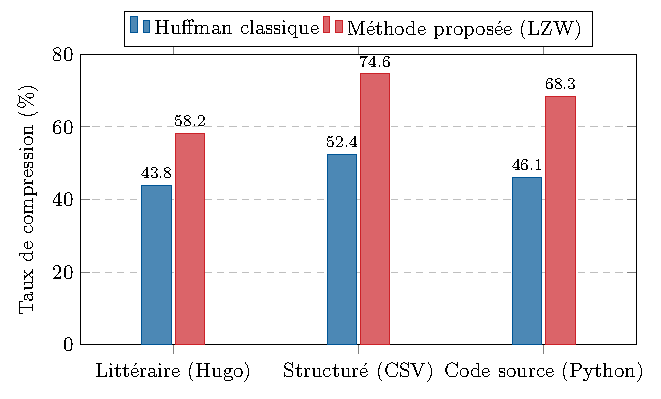
\includegraphics[width=0.75\textwidth]{figure_performances.pdf}
    \caption{Courbe ou histogramme comparatif des performances obtenues selon la méthode testée. Veillez à expliciter la légende et les unités employées.}
    \label{fig:exemple_figure}
\end{figure}

% ==============================================================================
% 3. CONCLUSION
% ==============================================================================
\section{Conclusion}
\label{sec:conclusion}
Résumez ici les principaux constats de votre travail pratique, la conformité de vos résultats face aux objectifs initiaux et les recommandations d'ingénierie qui en découlent.

% ==============================================================================
% RÉFÉRENCES
% ==============================================================================
\begin{thebibliography}{99}
    \bibitem{ref1}
    A.~Auteur, « Titre de l'article ou de la publication », \textit{Nom de la Revue ou Conférence}, vol.~10, no.~3, pp.~120--130, 2023.
    
    \bibitem{ref2}
    B.~Smith et C.~Jones, \textit{Titre du manuel de référence ou de la documentation}, 3e éd., Éditeur, 2024.
\end{thebibliography}

% ==============================================================================
% ANNEXES
% ==============================================================================
\newpage
\appendix
\section{Annexe : Données complémentaires et extraits de code}
\label{sec:annexe}

Cette annexe contient les données supplémentaires (calculs détaillés, tableaux de distribution étendus) ainsi que les extraits de code source clés développés pour le travail pratique.

\begin{lstlisting}[language=Python, caption={Exemple d'extrait de code source pour le traitement multimédia.}]
# Exemple d'extrait de code developpe par les etudiants
def traitement_multimedia(fichier_entree: str, fichier_sortie: str):
    """
    Fonction principale de traitement ou de compression des donnees.
    """
    # Inserer ici les instructions cles de votre algorithme
    print(f"Traitement de {fichier_entree} vers {fichier_sortie}")
\end{lstlisting}

\end{document}
